
\documentclass[12pt]{article}
\usepackage{amsmath}
\usepackage{graphicx}
\usepackage{hyperref}
\usepackage{listings}
\usepackage{color}
\usepackage{pythonhighlight}

\title{Operating System Course Report - First Half of the Semester}
\author{B class}
\date{\today}

\begin{document}
	
	\maketitle
	\newpage
	\tableofcontents
	\newpage
	
	\section{Introduction}
	This report summarizes the topics covered during the first half of the Operating System course. It includes theoretical concepts, practical implementations, and assignments. The course focuses on the fundamentals of operating systems, including system architecture, process management, CPU scheduling, and deadlock handling.
	
	\section{Course Overview}
	\subsection{Objectives}
	The main objectives of this course are:
	\begin{itemize}
		\item To understand the basic components and architecture of a computer system.
		\item To learn process management, scheduling, and inter-process communication.
		\item To explore file systems, input/output management, and virtualization.
		\item To study the prevention and handling of deadlocks in operating systems.
	\end{itemize}
	
	\subsection{Course Structure}
	The course is divided into two halves. This report focuses on the first half, which covers:
	\begin{itemize}
		\item Basic Concepts and Components of Computer Systems
		\item System Performance and Metrics
		\item System Architecture of Computer Systems
		\item Process Description and Control
		\item Scheduling Algorithms
		\item Process Creation and Termination
		\item Introduction to Threads
		\item File Systems
		\item Input and Output Management
		\item Deadlock Introduction and Prevention
		\item User Interface Management
		\item Virtualization in Operating Systems
	\end{itemize}
	
	\section{Topics Covered}
	
	\subsection{Basic Concepts and Components of Computer Systems}
	This section explains the fundamental components that make up a computer system, including the CPU, memory, storage, and input/output devices.
	
	\subsection{System Performance and Metrics}
	This section introduces various system performance metrics used to measure the efficiency of a computer system, including throughput, response time, and utilization.
	
	\subsection{System Architecture of Computer Systems}
	Describes the architecture of modern computer systems, focusing on the interaction between hardware and the operating system.
	
	\subsection{Process Description and Control}
	Processes are a central concept in operating systems. This section covers:
	\begin{itemize}
		\item Process states and state transitions
		\item Process control block (PCB)
		\item Context switching
	\end{itemize}
	
	\subsection{Scheduling Algorithms}
	This section covers:
	\subsubsection{First-Come, First-Served (FCFS)}
	Pendekatan paling sederhana untuk menjadwalkan proses adalah dengan menggunakan antrian FIFO (first-in, first-out). Proses baru masuk ke bagian akhir antrian. Ketika penjadwal perlu menjalankan sebuah proses, ia akan memilih proses yang ada di kepala antrian. Penjadwal ini bersifat non-preemptive, artinya proses yang sedang berjalan tidak bisa dihentikan sampai selesai. Jika proses harus menunggu I/O (input/output), ia akan masuk ke status waiting, dan penjadwal akan memilih proses berikutnya dari kepala antrian. Setelah I/O selesai dan proses yang menunggu siap untuk dijalankan kembali, ia akan dimasukkan ke bagian akhir antrian.
	
	Dengan first-come, first-served scheduling, proses yang memiliki burst CPU yang panjang akan memblokir proses lainnya, sehingga meningkatkan waktu turnaround (waktu total dari awal hingga akhir proses). Selain itu, ini juga bisa mengurangi throughput keseluruhan, karena proses I/O yang sedang menunggu mungkin sudah selesai, namun proses CPU-bound yang panjang masih berjalan. Akibatnya, perangkat (I/O) tidak digunakan secara efektif. Untuk meningkatkan throughput, akan lebih baik jika penjadwal bisa sementara menjalankan proses I/O-bound, sehingga proses tersebut bisa berjalan sebentar, meminta I/O, dan kemudian menunggu penyelesaian I/O tersebut.
	
	Karena proses CPU-bound tidak bisa dipreempt, ini juga berdampak buruk pada performa interaktif, karena proses interaktif tidak akan dijadwalkan sampai proses CPU-bound tersebut selesai.
		\begin{figure} [h]
			\centering
			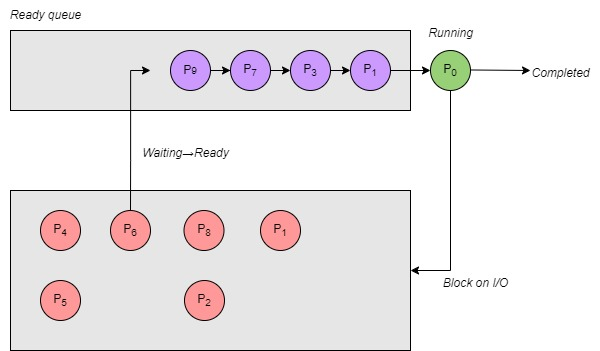
\includegraphics[width=0.5\textwidth]{assets/FCFS2.jpg}
			\label{fig:diagram}
		\end{figure}
		
	\subsubsection*{Karakteristik FCFS}
	\begin{itemize}
		\item FCFS mendukung penjadwalan CPU non-preemptive dan preemptive.
		\item Proses dieksekusi berdasarkan prinsip First-come, First-serve.
		\item Algoritma ini mudah diimplementasikan dan digunakan.
		\item FCFS kurang efisien dari segi kinerja karena waktu tunggu rata-ratanya cenderung tinggi.		
	\end{itemize}
		
	\subsubsection*{Algoritma Penjadwalan FCFS}
	Waktu tunggu untuk proses pertama adalah 0 karena proses tersebut dieksekusi pertama. Waktu tunggu untuk proses berikutnya dapat dihitung dengan rumus:
	
	\[
	wt[i] = (at[i–1] + bt[i–1] + wt[i–1]) – at[i]
	\]
	dimana:
	\begin{itemize}
		\item $wt[i]$ = waktu tunggu proses saat ini
		\item $at[i-1]$ = waktu kedatangan proses sebelumnya
		\item $bt[i-1]$ = burst time proses sebelumnya
		\item $wt[i-1]$ = waktu tunggu proses sebelumnya
		\item $at[i]$ = waktu kedatangan proses saat ini
	\end{itemize}
	
	Waktu tunggu rata-rata dapat dihitung dengan rumus:
	
	\[
	\text{Average Waiting Time} = \frac{\text{Total waktu tunggu}}{\text{Jumlah proses}}
	\]
	
	\subsubsection*{Kelebihan FCFS}
	\begin{itemize}
		\item Merupakan bentuk paling sederhana dan dasar dari algoritma penjadwalan CPU.
		\item Mudah diimplementasikan.
		\item Cocok untuk sistem batch di mana waktu proses yang lama biasanya dapat diterima.
	\end{itemize}
	
	\subsubsection*{Kekurangan FCFS}
	\begin{itemize}
		\item Karena ini adalah algoritma non-preemptive, proses akan berjalan hingga selesai tanpa bisa dihentikan.
		\item Waktu tunggu rata-rata dalam FCFS jauh lebih tinggi dibandingkan algoritma lainnya.
		\item Mengalami efek (Convoy effect), yaitu proses besar menghalangi proses yang lebih kecil.
		\item Tidak efisien karena terlalu sederhana.		
		\item Proses yang berada di akhir antrian harus menunggu lebih lama.		
		\item Tidak cocok untuk sistem operasi time-sharing di mana setiap proses harus mendapatkan jatah waktu CPU yang sama.	
	\end{itemize}
	
	\subsubsection*{Referensi}
	\begin{itemize}
		\item GeeksforGeeks. (n.d.-a). First Come First Serve | CPU scheduling (non-preemptive). Retrieved October 1, 2024, from https://www.geeksforgeeks.org/first-come-first-serve-cpu-scheduling-non-preemptive/
		
		\item GeeksforGeeks. (n.d.-b). Program for FCFS CPU scheduling | Set 1. Retrieved October 1, 2024, from https://www.geeksforgeeks.org/program-for-fcfs-cpu-scheduling-set-1/
	\end{itemize}
		
	\subsubsection{Shortest Job Next (SJN)}
	\subsubsection{Round Robin (RR)}
	It explains how these algorithms are used to allocate CPU time to processes.
	
	\subsection{Process Creation and Termination}
	Details how processes are created and terminated by the operating system, including:
	\begin{itemize}
		\item Process spawning
		\item Process termination conditions
	\end{itemize}
	
	\subsection{Introduction to Threads}
	This section introduces the concept of threads and their relation to processes, covering:
	\begin{itemize}
		\item Single-threaded vs. multi-threaded processes
		\item Benefits of multithreading
	\end{itemize}
	
	\subsection{File Systems}
	File systems provide a way for the operating system to store, retrieve, and manage data. This section explains:
	\begin{itemize}
		\item File system structure
		\item File access methods
		\item Directory management
	\end{itemize}
	
	\subsection{Input and Output Management}
	Input and output management is key for handling the interaction between the system and external devices. This section includes:
	\begin{itemize}
		\item Device drivers
		\item I/O scheduling
	\end{itemize}
	
	\subsection{Deadlock Introduction and Prevention}
	Explores the concept of deadlocks and methods for preventing them:
	\begin{itemize}
		\item Deadlock conditions
		\item Deadlock prevention techniques
	\end{itemize}
	
	\subsection{User Interface Management}
	This section discusses the role of the operating system in managing the user interface. Topics covered include:
	\begin{itemize}
		\item Graphical User Interface (GUI)
		\item Command-Line Interface (CLI)
		\item Interaction between the user and the operating system
	\end{itemize}
	
	\subsection{Virtualization in Operating Systems}
	Virtualization allows multiple operating systems to run concurrently on a single physical machine. This section explores:
	\begin{itemize}
		\item Concept of virtualization
		\item Hypervisors and their types
		\item Benefits of virtualization in modern computing
	\end{itemize}
	
	\section{Assignments and Practical Work}
	\subsection{Assignment 1: Process Scheduling}
	Students were tasked with implementing various process scheduling algorithms (e.g., FCFS, SJN, and RR) and comparing their performance under different conditions.
	
	\subsection{Assignment 2: Deadlock Handling}
	In this assignment, students were asked to simulate different deadlock scenarios and explore various prevention methods.
	
	\subsection{Assignment 3: Multithreading and Amdahl's Law}
	\subsubsection{Group 5}
	Tentukan peningkatan kecepatan teoritis (speedup) menggunakan Hukum Amdahl dengan beberapa thread, dan bandingkan hasilnya dengan waktu eksekusi yang diukur.Program harus memenuhi spesifikasi sebagai berikut :
	\begin{itemize}
		\item Buatlah sebuah program Python yang menghitung faktorial dari beberapa angka secara paralel menggunakan multithreading. Setiap thread akan menghitung faktorial dari satu angka yang berbeda.
		\item Gunakan 1 thread, 2 thread, dan 4 thread untuk melakukan perhitungan dan catat waktu eksekusi dari setiap percobaan.
		\item Terapkan Hukum Amdahl dengan asumsi bahwa 90 persen dari tugas dapat diparalelkan. Hitung peningkatan kecepatan teoretis untuk penggunaan 2 dan 4 thread.
		Bandingkan waktu eksekusi yang diukur dengan speedup teoretis yang dihitung menggunakan Hukum Amdahl.
		
		\item Jelaskan perbedaan antara peningkatan kecepatan yang sebenarnya dan yang dihitung secara teoretis.
	\end{itemize}
	\begin{python}
		
		import threading
		import os
		import math
		import time
		
		def hitung_faktorial(angka):
		print(f"Thread {threading.current_thread().name} dimulai dengan ID: {threading.current_thread().name}")
		hasil = math.factorial(angka)
		print(f"Faktorial dari {angka} adalah: {hasil}")
		print(f"Thread {threading.current_thread().name} selesai")
		
		def ukur_waktu_eksekusi(thread_count):
		start_time = time.time()
		
		threads = []
		for i in range(thread_count):
		t = threading.Thread(target=hitung_faktorial, args=(i+5,), name=f"Thread-{i+1}")
		threads.append(t)
		t.start()
		
		for t in threads:
		t.join()
		
		end_time = time.time()
		
		return end_time - start_time
		
		def amdahls_law(P, N):
		return 1 / ((1 - P) + (P / N))
		
		if __name__ == "__main__":
		P = 0.9  
		
		print(f"ID dari proses utama: {os.getpid()}")
		
		waktu_serial = ukur_waktu_eksekusi(1)
		print(f"Waktu eksekusi tanpa multithreading: {waktu_serial:.4f} detik")
		
		waktu_parallel_2 = ukur_waktu_eksekusi(2)
		print(f"Waktu eksekusi dengan 2 thread: {waktu_parallel_2:.4f} detik")
		
		speedup_2 = amdahls_law(P, 2)
		print(f"Speedup teoretis dengan 2 thread: {speedup_2:.2f} kali lebih cepat")
		
		waktu_parallel_4 = ukur_waktu_eksekusi(4)
		print(f"Waktu eksekusi dengan 4 thread: {waktu_parallel_4:.4f} detik")
		
		speedup_4 = amdahls_law(P, 4)
		print(f"Speedup teoretis dengan 4 thread: {speedup_4:.2f} kali lebih cepat")
		
		print("Perhitungan faktorial selesai")
		
	\end{python}
	
	
	
	\subsection{Assignment 4: Simple Command-Line Interface (CLI) for User Interface Management}
	Students were tasked with creating a simple **CLI** for user interface management. The CLI should support basic commands such as file manipulation (creating, listing, and deleting files), process management, and system status reporting.
	
	\subsection{Assignment 5: File System Access}
	In this assignment, students implemented file system access routines, including:
	\begin{itemize}
		\item File creation and deletion
		\item Reading from and writing to files
		\item Navigating directories and managing file permissions
	\end{itemize}
	
	\section{Conclusion}
	The first half of the course introduced core operating system concepts, including process management, scheduling, multithreading, and file system access. These topics provided a foundation for more advanced topics to be covered in the second half of the course.
	
\end{document}
